\documentclass[twoside,11pt]{article}

\usepackage{blindtext}
\usepackage{natbib}
\setcitestyle{square, numbers}
\usepackage{hyperref}
\usepackage{graphicx}
\usepackage{float}
\usepackage{svg}
\usepackage{amsmath}
\usepackage{amssymb}

\hypersetup{
    colorlinks=true,
    linkcolor=blue,
    citecolor=blue,
    urlcolor=blue
}

% Any additional packages needed should be included after jmlr2e.
% Note that jmlr2e.sty includes epsfig, amssymb, natbib and graphicx,
% and defines many common macros, such as 'proof' and 'example'.
%
% It also sets the bibliographystyle to plainnat; for more information on
% natbib citation styles, see the natbib documentation, a copy of which
% is archived at http://www.jmlr.org/format/natbib.pdf

% Available options for package jmlr2e are:
%
%   - abbrvbib : use abbrvnat for the bibliography style
%   - nohyperref : do not load the hyperref package
%   - preprint : remove JMLR specific information from the template,
%         useful for example for posting to preprint servers.
%
% Example of using the package with custom options:
%
% \usepackage[abbrvbib, preprint]{jmlr2e}


% \newcommand{\dataset}{{\cal D}}
% \newcommand{\fracpartial}[2]{\frac{\partial #1}{\partial  #2}}

% Heading arguments are {volume}{year}{pages}{date submitted}{date published}{paper id}{author-full-names}

\usepackage{lastpage}


% 

\begin{document}



\title{Quantum dots Energy levels}

\author{
        \name Khaled Hasan \\ \email khaledoqab@gmail.com \\ \vspace{2cm}\\
        supervised by:\\ Prof. Khalid Eid\\
        \vspace{10cm}
       \addr Department of Physics\\
       Birzeit University
       }
% \editor{My editor}

\maketitle
\newpage
\begin{abstract}%   <- trailing '%' for backward compatibility of .sty file
    Quantum dots is Nano-scale technology that makes use of the quantum confinement due to its small size that is confined in 3 dimensions to exhibit interesting optical and electrical properties, furthermore, their relative large size compared to atoms enables researchers and manufacturers to tune and control these properties, by controlling the size, shape and materials that make up these dots. In this paper I will give an overview of the manufacturing methods (to shine light on the ways that their properties are controlled), then I will provide few theoretical results explaining how the energy changes with size, and explore the methods used to solve for the resulting confined discrete energy states. Then I will present few experimental results, from researchers who have attempted to manipulate the dots energy spectra. Last I will give a brief insight on the future and where the recent researches are heading. 
\end{abstract}


\section{Introduction}

quantum dots are zero dimensional semiconducting nano-structures (has sizes of order $\mathcal{O}((10nm)^3)$), their small sizes are responsible for certain optical and electronic properties via quantum effects, also, their relatively big size (compared to that of single atoms) makes it possible (or easier) to control and change said properties, which is why they are sometimes called \textbf{artificial atoms}.\\
quantum dots are zero dimensional in the sense that electrons (or holes alike) motion is restricted in the 3 dimensions, this restriction on the electron's motion leads to a behaviour similar to that of the popular infinite well case in quantum mechanics, which is why quantum dots are sometimes modeled by quantum box or spherical wells.\\
For the purpose of trapping or restricting an electron in a vacuum a volume of $1nm$ across is required, however, due to the electrostatic potential of atoms in the used semiconductor reduce the inertia of the electron and therefore reduced the effective mass $(m_{eff})$, the reduction of the effective mass increases the wavelength of the electron and therefore increases the length under which confinement effects take place . leading to the possibility of creating larger quantum dots that are easier to make and modify. \cite{reed1993quantum}\\
As previously mentioned, quantum dots are made semiconducting materials, usually this material is some variation of \textbf{GaAs} (such as \textbf{InGaAs}), rather than silicon, due to the smaller $m_{eff}$ in \textbf{GaAs} compared to \textbf{Si} as well as its enhanced ability to grow  layered structures. However, lately more efforts and researches has been dedicated towards carbon and graphine quantum dots these will be adressed later.\cite{shur1989gallium}\\
The special properties of quantum dots lead to many interesting applications, such as diode lazers, $1$ electron transistors, sensors and Display technologies. The essence of these applications is the control over \textbf{energy levels} of the \textbf{QD}. In this paper, I will focus on the determination and manipulation of the energy levels of quantum dots.

\section{Production}
there are many ways to produce quantum dots, the production process of quantum dots contributes heavily to the properties of QDs. By adjusting the size, shape, material and annealing temperature of the QDs, one can manipulate the energy levels of the QDs as well as controlling the line-width of the photoluminescence peaks and intersublevel spacing energies. Here I will consider three production methods methods:

    \subsection{Epitaxial growth (Stranski–Krastanow mode)}
    In Molecular-Beam Epitaxy (MBE), a substrate is positioned in a vacuum or ultra-vacuum chamber, where several effusion cells with the desired substance (in this case, (InAs) and GaAs), these effusion cells contain heating coils that upon heating up will start emitting beams of molecules targeted towards the substrate (check figure \ref{MBE apparatus}), by controlling the temperature one can control the rate of deposition on the substrate, and thus manipulate the sizes and shpes of QDs, by this method one can form thin films and small nano-islands on the substrates. In the Stranski–Krastanow mode 2D nano-surfaces are formed to a certain thickness, then 3D islands start forming.\\ Quantum dots are formed by first creating buffer undoped layers of the semi-conductor (GaAs) followed by the QDs material (InAs) which is then capped by the undoped semi-conductor, each step is performed at a tuned temperature \cite{hsu2000tuning}.
    
    % include this in presentation: The main limitations of this method are the cost of fabrication and the lack of control over positioning of individual dots.
    
    \begin{figure}[h]
        \centering
        \includesvg[scale = 0.08]{MBE.svg}
        \caption{MBE apparatus\\ \small{By Vegar Ottesen - Own work, CC BY 3.0, https://commons.wikimedia.org/w/index.php?curid=16957521}}
        \label{MBE apparatus}
    \end{figure}
        
    \subsection{Electrical gating}
    In this method A layer of the doped semiconductor is grown on top of a layer of an undoped semiconductor using (MBE), electrons will accumulate on the junction interface, restricting the motion in the vertical direction (typically $50$ - $100$nm below the surface). Then nano electron electrodes (or gates) are formed at the top of the structure by electron-beam lithography, by applying a negative voltage to the gates, the electrons on the interface between the layers are depleted, it can also be thought of as forming a potential wall in the gate region, and thus restricting electron motion in the lateral direction as well to small region between the gates forming a quantum dot, while outside the gates region is a 2D electrons see which is connected to the dot by point contacts (see figure \ref{one electron transistor})\cite{alhassid2000statistical}.
    
    \begin{figure}[h]
        \centering
        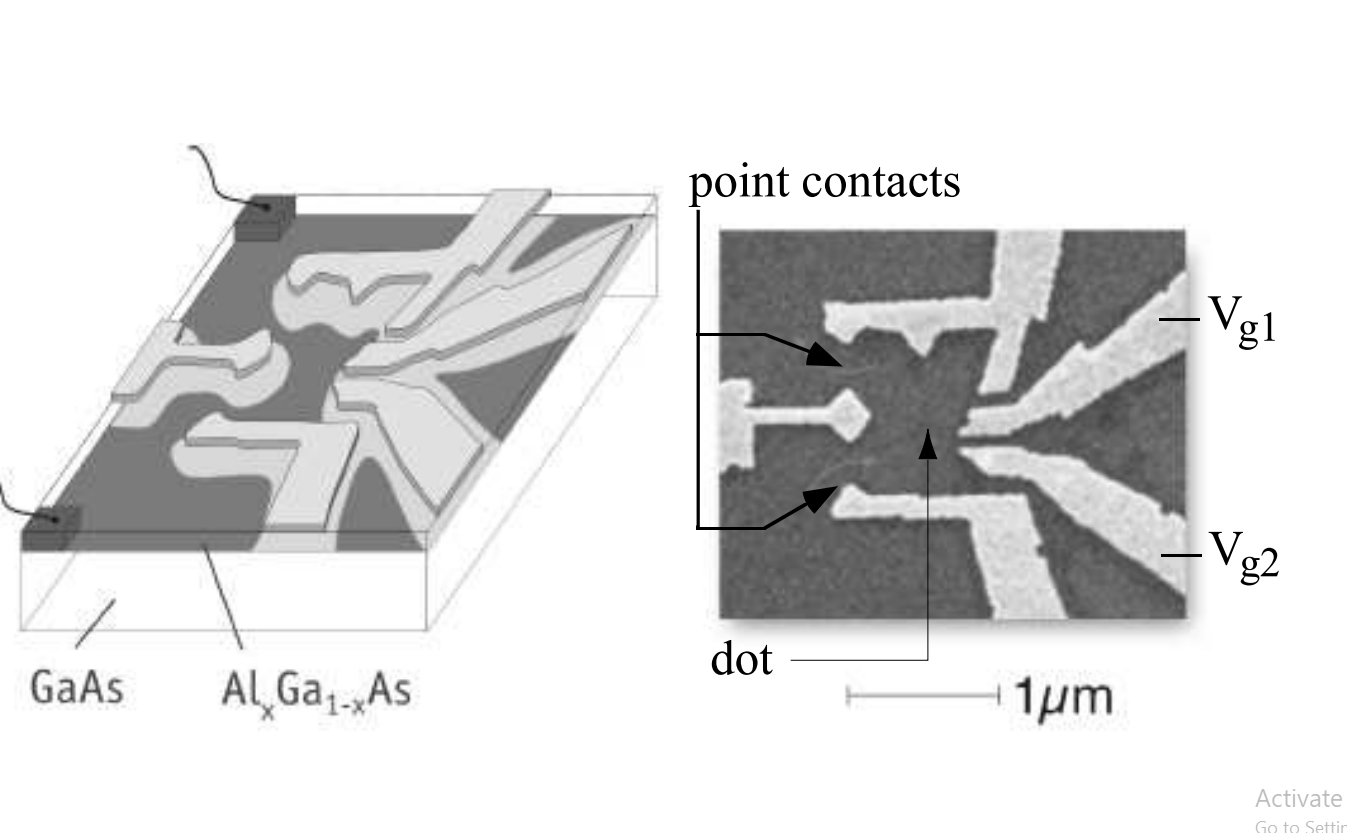
\includegraphics[scale = 0.35]{2024-04-06.png}
        \caption{a quantum dot used by Folk et al.(1996), light regions are were gates are placed, and from which electrons are depleted, whereas dark regions are the quantum dot (trapped in the middle) and the 2D electron sea (source and drain)}
        \label{one electron transistor}
    \end{figure}
    
    One of the key advantages of these quantum dots is the flexibility in terms of shape and size, The shape and size of the dot can be controlled
    by voltages $Vg1$ and $Vg2$ show in figure \ref{one electron transistor}, which as a result will change some of the characteristics of the dot.\\
        \subsubsection{Single electron transistor}
        Under certain tunneling conditions, electrons from the $2D$ electron reservoirs in contact with the dot in figure \ref{one electron transistor} can tunnel through the quantum dot, and from the dot to the adjacent region. The tunneling is blocked by the Coulomb blockade, which is the state in which the first excited state $E_{(N+1)}$ after the Fermi level energy level $(N)$ in the dot is higher than that in the adjacent reservoirs $E_{N+1} > \mu$, while the Fermi energy is smaller than the reservoir $\mu > E_N$, so that no tunneling from the dot to the reservoirs occurs, and as a result no current will flow in the dots.\\ However, if the energy of the dot decrease and a potential difference is introduced between both reservoirs (call them drain and source) such that $\mu_d<E_{N+1}<\mu_s$ then current will flow from the source to the drain (see figure \ref{coloumb blockade}). This behaviour is similar to that of a transistor, where no current flows from source to drain unless some voltage is introduced to the gate, which makes the dot a nano-transistor, this sort of transistors is called single electron transistor, since it only uses single electron which tunnels to the first free state and then to the drain.\\With increasing gate potential, the conductivity $G=I/V_{sd}$ will oscillate (as $E_n$ goes below $\mu_d$), this is called coulomb oscillation.
        
        \begin{figure}[h]
            \centering
            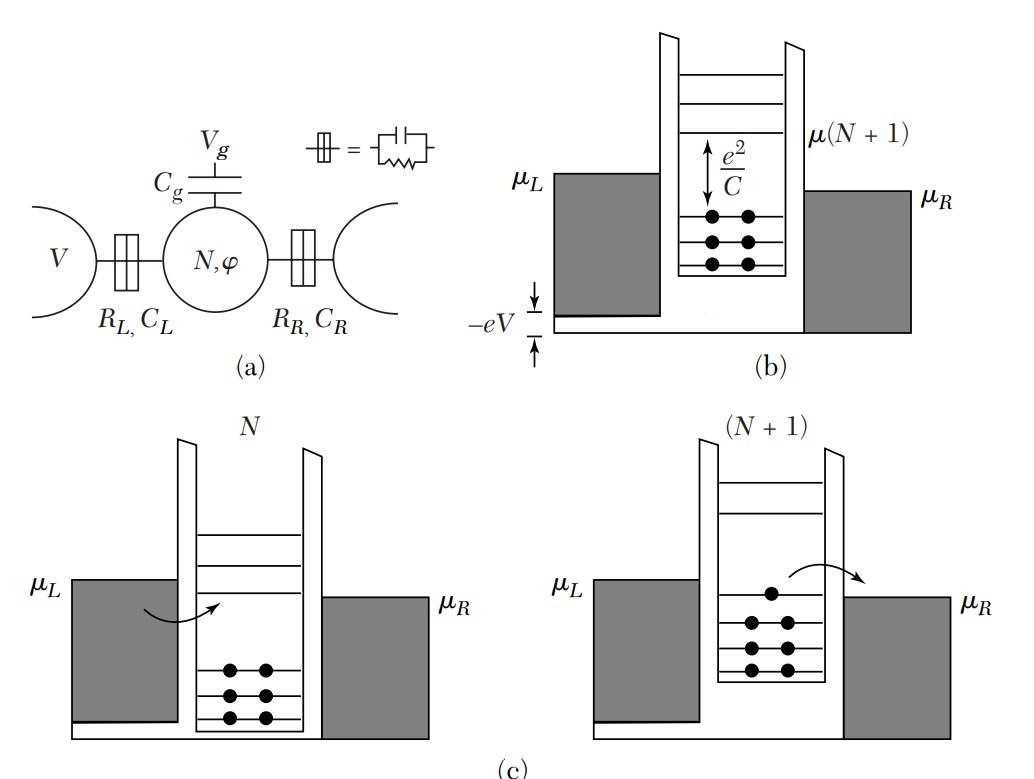
\includegraphics[scale = 0.4]{2024-04-06 (1).png}
            \caption{Figure from Kittel (a) quantum dot in contact with two metallic reservoirs and to a gate.Conditions of coulomb blockade, in (b) coulomb blockade (c) coulomb blockade lifted when the dot potential is lowered, allowing current to flow}
            \label{coloumb blockade}
        \end{figure}

    \subsection{Electron beam lithography}
    In this method, a semiconductor coated with resist and containing buried quantum dot material (this could be prepared using MBE) is scanned by electron-beam lithography, which removes the resist from a small desired region, the whole surface is then coated with metallic layer, then the resist will be removed (alongside the coating metallic layer), which keeps only the desired part with no resist protected, using reactive ions to etch away the chip except where it is protected by metal, as a result, the quantum dot below the determined region will be isolated.\cite{reed1993quantum}

    \subsection{Colloidal Synthesis}
    % If time permits
    This is a promising method for large scale production of QDs using liquid phase epitaxial growth, By rapid injection of a certain solution of one or more organometallic precursor into a hot mixture of organic solvents, then fast mixing of the mixture solution. These processes produce high-quality QDs with optimal physical and chemical characteristics under precise control of the reaction parameters such as precursor injection speed, stirring rate, and temperature (which are difficult to control) \cite{pu2018colloidal}.


\section{Energy Manipulation}

    \subsection{Simple Quantum well Modelling}
    Quantum dots are usually modeled as 3D quantum wells, assuming a simple spherical shape of the dot with radius $R$, the solution become that of a spherical infinite well:
    \begin{equation}
        \mathcal{\psi}(r,\theta,\phi) = Y_{l,m}(\theta,\phi) j_l\left(\beta_{n, l}\frac{r}{R}\right)(r)
        \label{simple model}
    \end{equation}
    with energies $E_{n, l, m} = E_{n, l}$ given by
    \begin{equation}
        E_{n, l} = \frac{\hbar^2\beta_{n, l}^2}{2m_{eff}R^2}
        \label{simple model energy}
    \end{equation}
    This perfectly spherical model was used to fit experimental data in \cite{10.1063/1.3284083} where it performed even better than the finite well method, where the energy errors are smaller than $3\%$ (this was most likely due to errors in determining the finite well potential barrier). These models can also be used on different dots shapes, but these shapes will not have the nice analytical form of \ref{simple model energy}, To further depict this I will use numerical methods to solve the (InAs/GaAs) system following from \cite{marzin1994calculation}.\\
    We will make the following approximations:
    
    \begin{enumerate}
        \item The InAs crystal is conic with radius $r_c$ and height $h$.
        \item The effective masses is material independent.
        \item material independent effective masses
    \end{enumerate}
    
    % \begin{figure}[h]
    %     \centering
    %     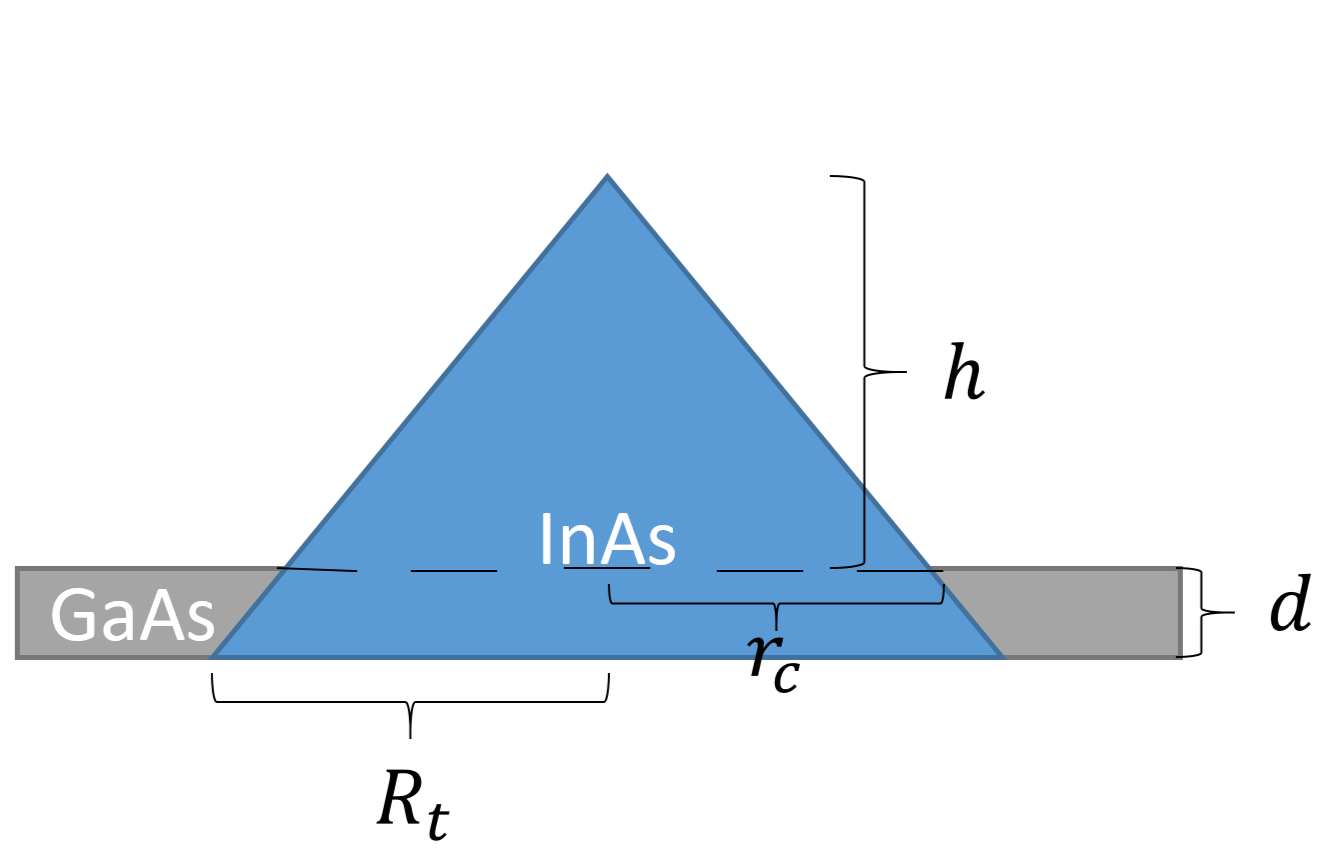
\includegraphics[scale = 0.25]{2024-04-07 (2).png}
    %     \caption{cross sectional view of InAs/GaAs unit}
    %     \label{InAs/GaAs}
    % \end{figure}

        \subsubsection{Numerical Solution}
        Then we can write the Hamiltonian as:
        \begin{equation}
            H = -\frac{\hbar^2}{2}\left( \frac{1}{m_z} \frac{\partial^2}{\partial z^2} + \frac{1}{m_r} \frac{1}{r} \frac{\partial}{\partial r} r \frac{\partial}{\partial r} + \frac{1}{r^2} \frac{\partial^2}{\partial \phi^2}\right) + V(r, z) 
        \end{equation}
        
        due to azimuthal quantization condition $\Phi = \exp(in\phi)$ and thus $P_{\phi} = -\frac{n}{m_\phi r^2}$:
        
        \begin{equation}
            H(r, z) = -\frac{\hbar^2}{2}\left( \frac{1}{m}\frac{\partial^2}{\partial z^2} + \frac{1}{m}\frac{1}{r}\frac{\partial}{\partial r} r \frac{\partial}{\partial r}\right) - \frac{n^2}{m r^2} + V(r, z) 
            \label{Hamiltonian}
        \end{equation}
        
        where $m = m_r = m_z = m_{\phi}$ is the effective mass.
        
        In \cite{marzin1994calculation} the authors made few more assumptions to use separability and obtain analytical approximation, and used numerical approach with product of Bessel and periodic functions, here, I will consider a different approach, I will turn equation \ref{Hamiltonian} into a matrix, and the Schrodinger equation into an eigenvalue problem.
        
        first redefine $r = r/R$ and $z = z/Z$ so that $r, z$ are dimensionless where $R, Z$ are big enough to be considered infinite (in this scenario, $Z = R = 40nm$)
        
        by desensitization of the above Hamiltonian:
        \begin{equation}
            \begin{split}
            H^{(i, j)}_{k, l} = & \frac{-\hbar^2}{2mR^2}e_{k, l}\left(\frac{\varepsilon^{i-1} -2\varepsilon^{i} + \varepsilon^{i+1}}{\Delta r^2} + \frac{\varepsilon^{i+1}-\varepsilon^{i-1}}{2r_i\Delta r} - \frac{n^2}{r_i^2}\varepsilon^{i}\right) \\
            & + \frac{-\hbar^2}{2mZ^2}e_{k, l}\left(\frac{\varepsilon^{j-1} -2\varepsilon^{j} + \varepsilon^{j+1}}{\Delta z^2}\right) + V(r_i, z_j)e_{k, l}\varepsilon^{(i, j)}
            \end{split}
        \end{equation}
        
        where $e_{k, l}, \varepsilon^{(i, j)}$ are meant to be the position basis and dual basis in the Hilbert space, where $i, k$ are indices over $r$ whereas $l, j$ are indices over $z$.
        \begin{equation}
            \vert \psi \rangle = \psi(r_i, z_j) e_{i, j}
        \end{equation}
        due to discretizarion in a finite grid of size $(N\times M)$, the following mapping could be made $(i, j) \to Ni + j = i$, $(k, l) \to Nk + l = k$
        
        \begin{equation}
            \begin{split}
            {H^i}_k = & \frac{-\hbar^2}{2mR^2}e_k \left(\frac{\varepsilon^{i-1} -2\varepsilon^{i} + \varepsilon^{i+1}}{\Delta r^2} + \frac{\varepsilon^{i+1}-\varepsilon^{i-1}}{2r_i\Delta r} - \frac{n^2}{r_i^2}\varepsilon^{i}\right) \\
            & + \frac{-\hbar^2}{2mZ^2}e_{k}\left(\frac{\varepsilon^{i-N} -2\varepsilon^{i} + \varepsilon^{i+N}}{\Delta z^2}\right) + V^i e_{k}\varepsilon^{i}
            \end{split}
            \label{H matrix}
        \end{equation}
        
        It is clear from equation \ref{H matrix} that $H$ is a matrix, with dimensions $NM \times NM$, since $NM$ is usually very large, $H$ is usually treated as a sparse matrix, the potential part can be simply extracted by the creating a diagonal matrix whose diagonal is the potential matrix elements reshaped to an array with length $NM$, whereas the kinetic energy operator can be obtained using Kronecker sum between the derivative operators, taking into account the boundary conditions, in the $P_z$ operator, $z$ is vanishing at edges, while the $P_r$ operator ensures vanishing at $r \to \infty$, and $\left.\frac{\partial \psi}{\partial \theta}\right|_{r = 0} = 0$, for this case, the derivative matrices should be modified as follows:
        \begin{equation}
            \begin{split}
                \partial^2_r [0, 0] =& -1\\
                \partial_r [0, 1] =& 0
            \end{split}
            \label{BCs}
        \end{equation}
        
        where
        \begin{equation}
            H = -\frac{\hbar^2}{2m_{\text{eff}}}\left[\left(\partial_r^2 + \text{diag}(1/r)\partial_r - \text{diag}(n^2/r^2)\right) \oplus \partial_z^2\right] + \text{diag}(V(r, phi))
            \label{comp eq}
        \end{equation}

        \subsubsection{Results}
        I used python to solve the Schrodinger equation whose Hamiltonian is \ref{comp eq}, I used scipy.sparse to define the matrices, and solve the eigenvalue problem with eigs function, notice that there is a randomness in the algorithm, so to obtain correct results find the smallest 6 or so eigenvalues (whose real part is minimum) and take the smallest for ground state energy, doing this the following result was obtained:
        \begin{figure}[h]
            \centering
            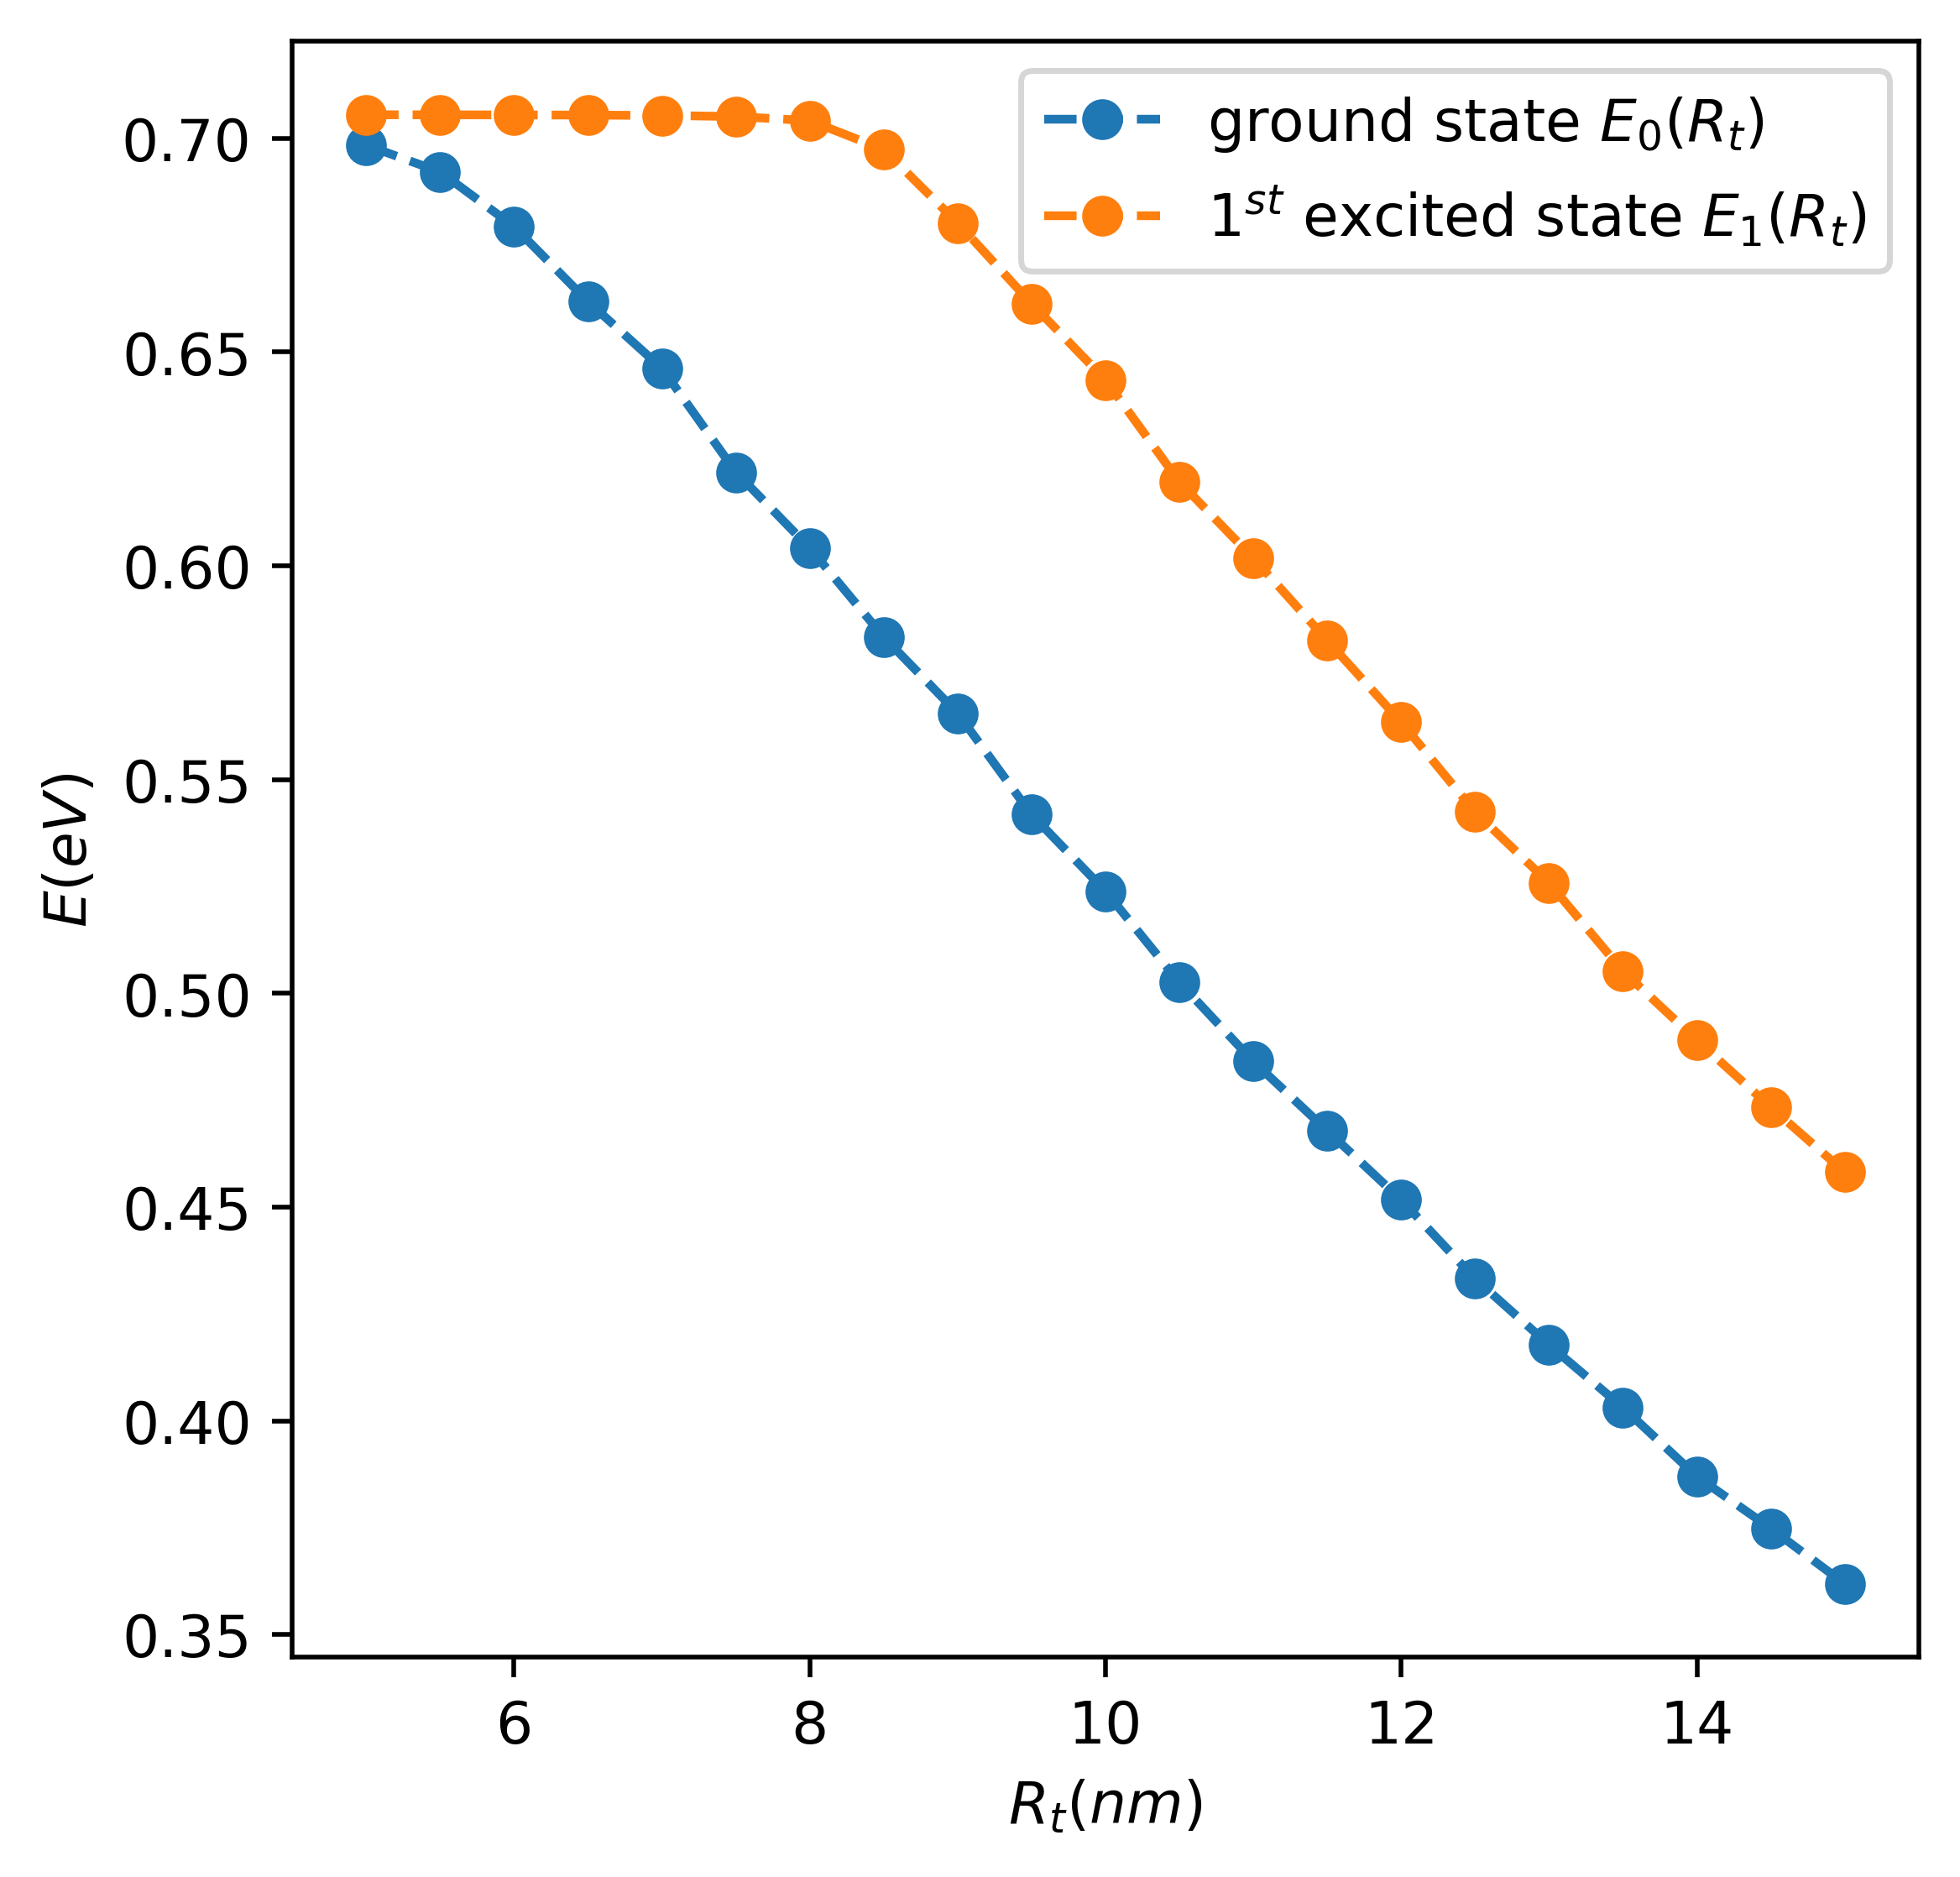
\includegraphics[scale = 0.5]{output.png}
            \caption{Conic InAs quantum dots ground and first excited states energies as a function of base radius (with base angle $= 12$ according to \cite{marzin1994calculation})}
            \label{fig my QD enegries}
        \end{figure}
    
        for comparison sake, I will include the results provided by \cite{marzin1994calculation}
        \begin{figure}[h]
            \centering
            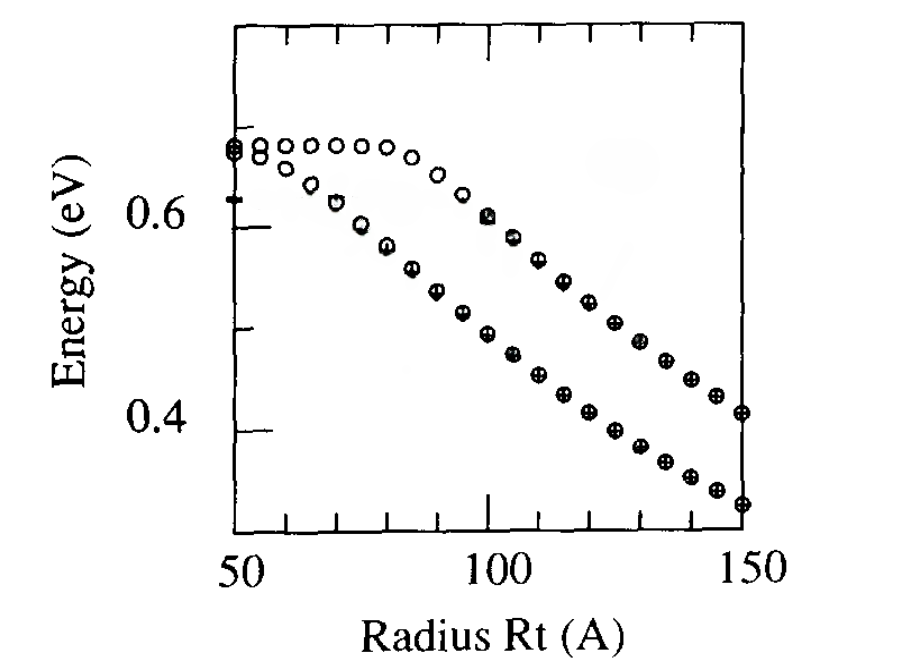
\includegraphics[scale = 0.4]{2024-04-17.png}
            \caption{Results from \cite{marzin1994calculation} for the calculations depicted in \ref{fig my QD enegries}}
            \label{results from origional paper}
        \end{figure}
    
    
        doing the same with heavy holes to obtain the transition energies between electrons and holes using light and heavy holes, which reflects the emission energies of the dots.
        \begin{figure}[h]
            \centering
            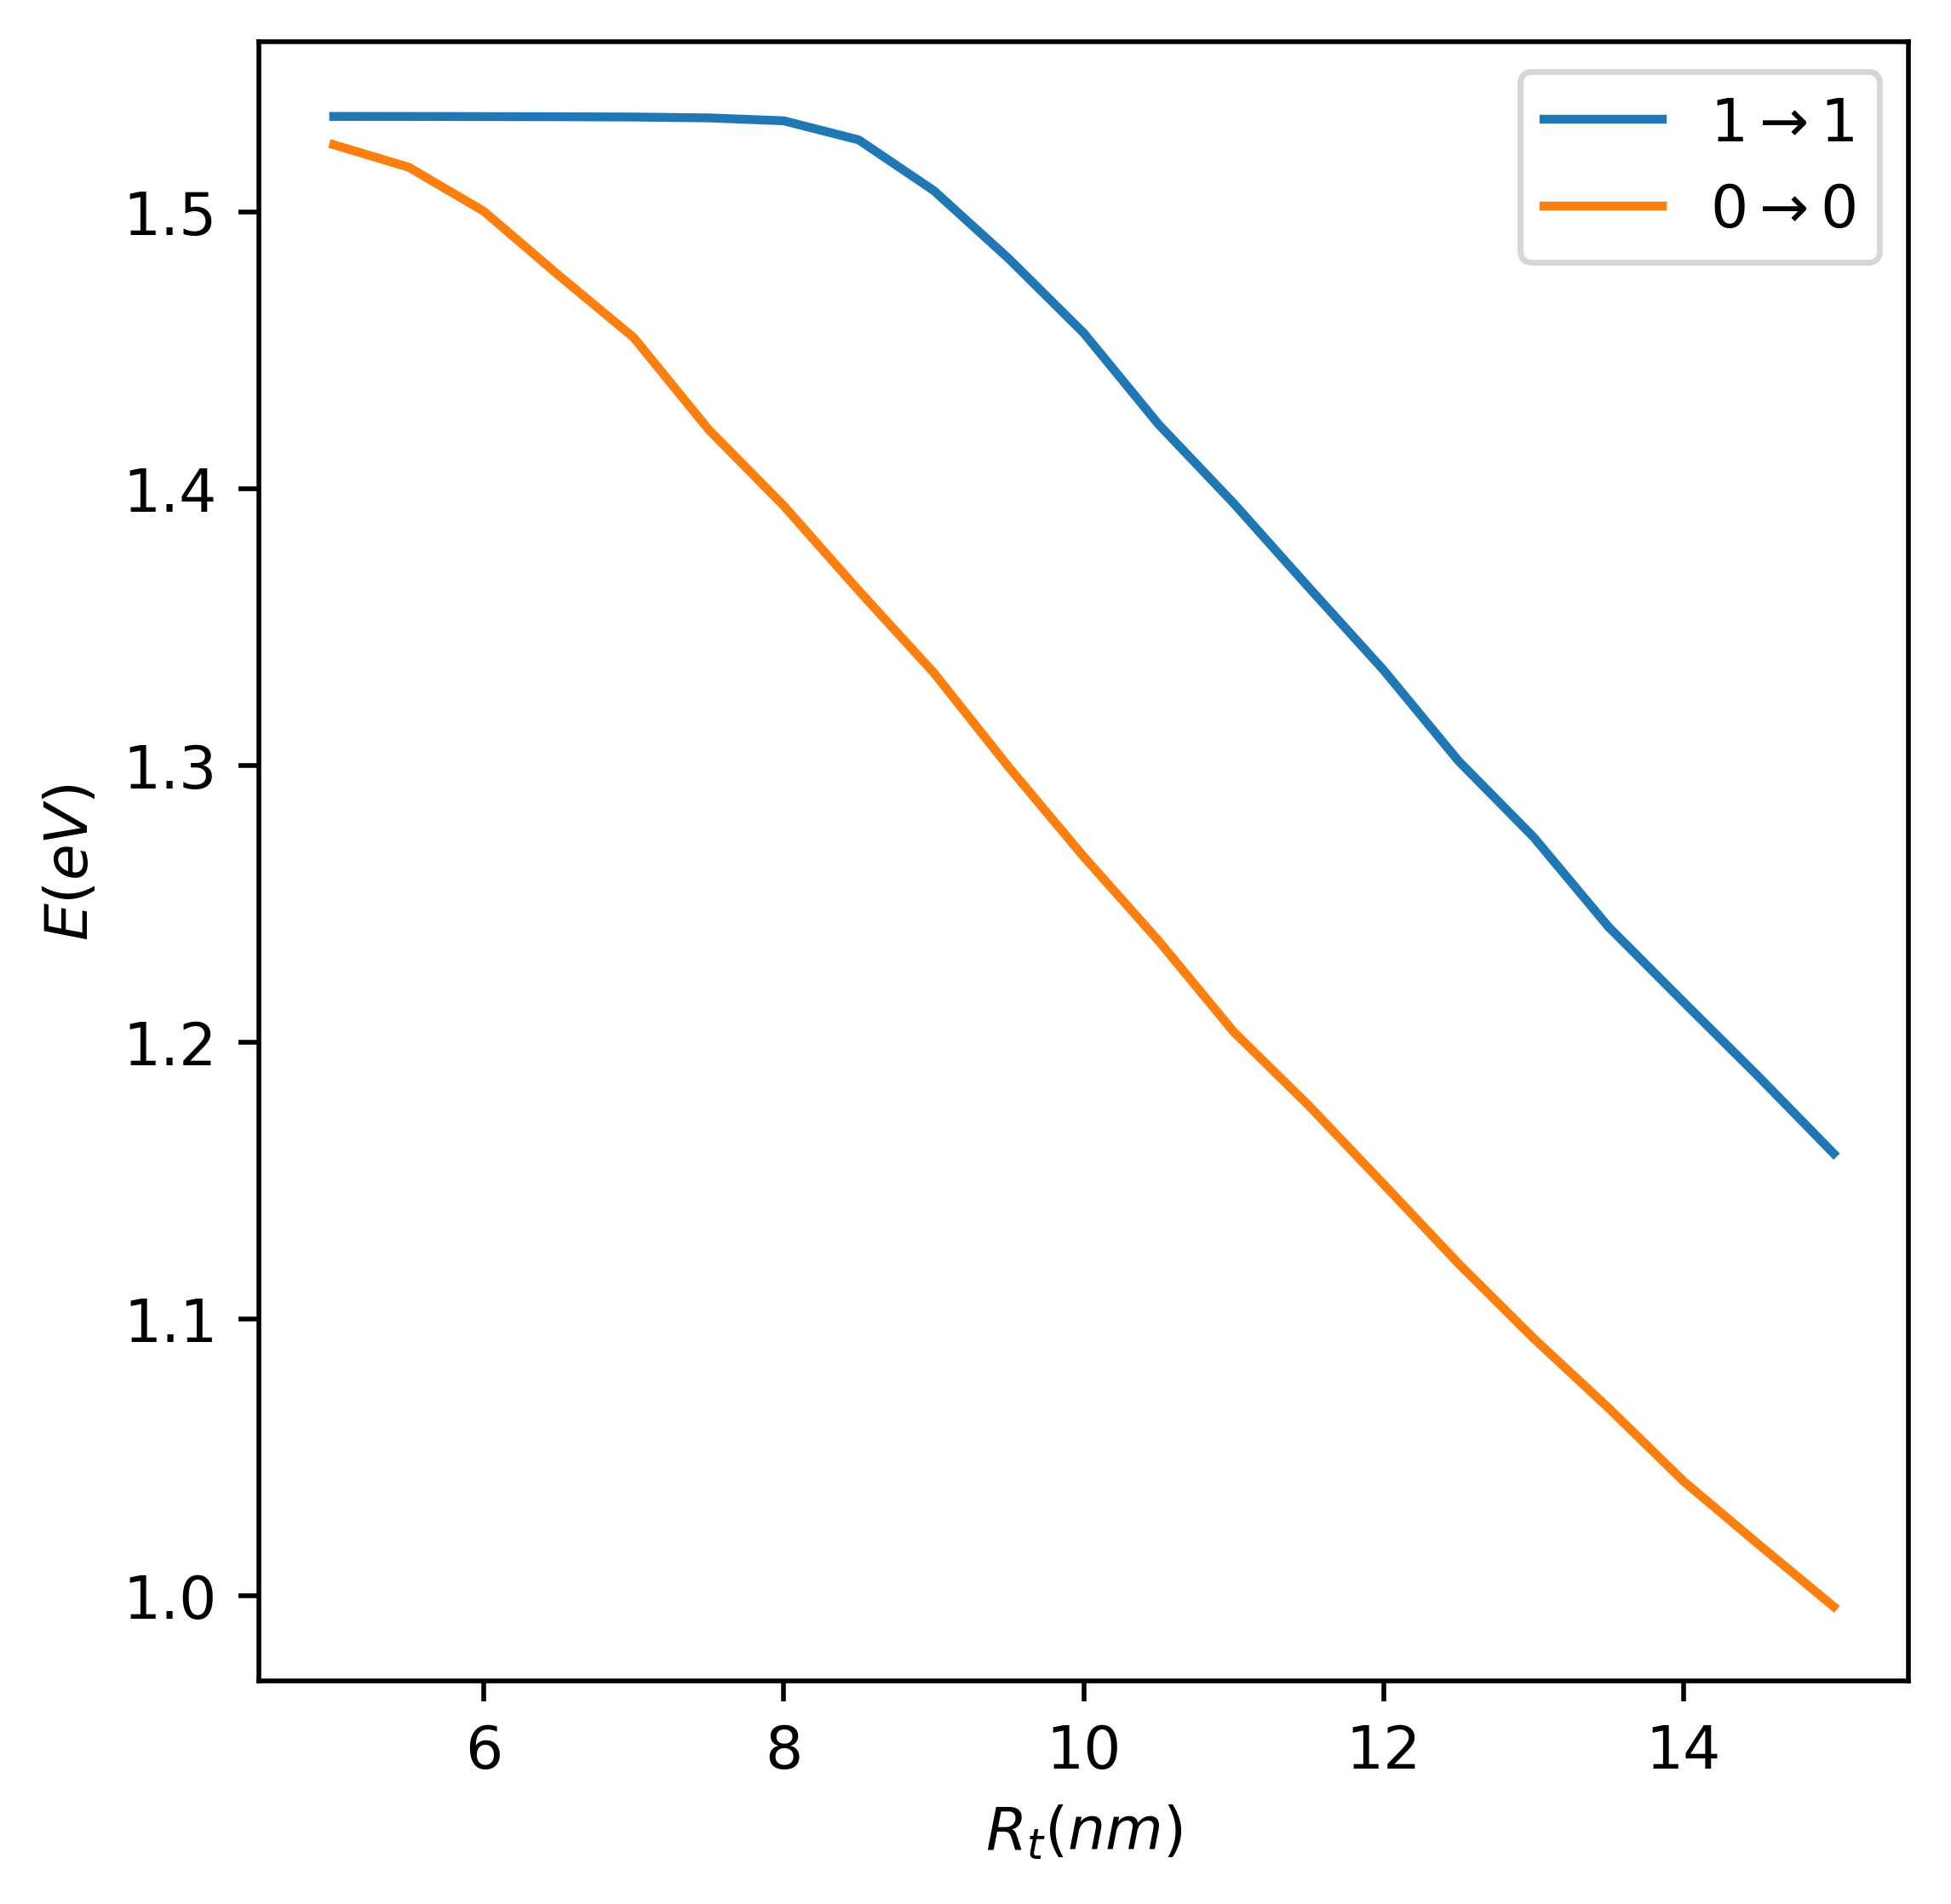
\includegraphics[scale = 0.5]{Transition Energies.png}
            \caption{first two transition energies of heavy holes, and first transition energy of light hole}
            \label{fig:transition energies}
        \end{figure}
    
        According to \cite{marzin1994calculation} these results have shown excellent agreement with the experiments using AFM and photoluminescence data to estimate low temperature energies and the corresponding geometry. We can also check how the ground state energies falls in proportion with $\prop a(r+b)^{-2}$ as depicted in figure \ref{fig: fitting}
        \begin{figure}[h]
            \centering
            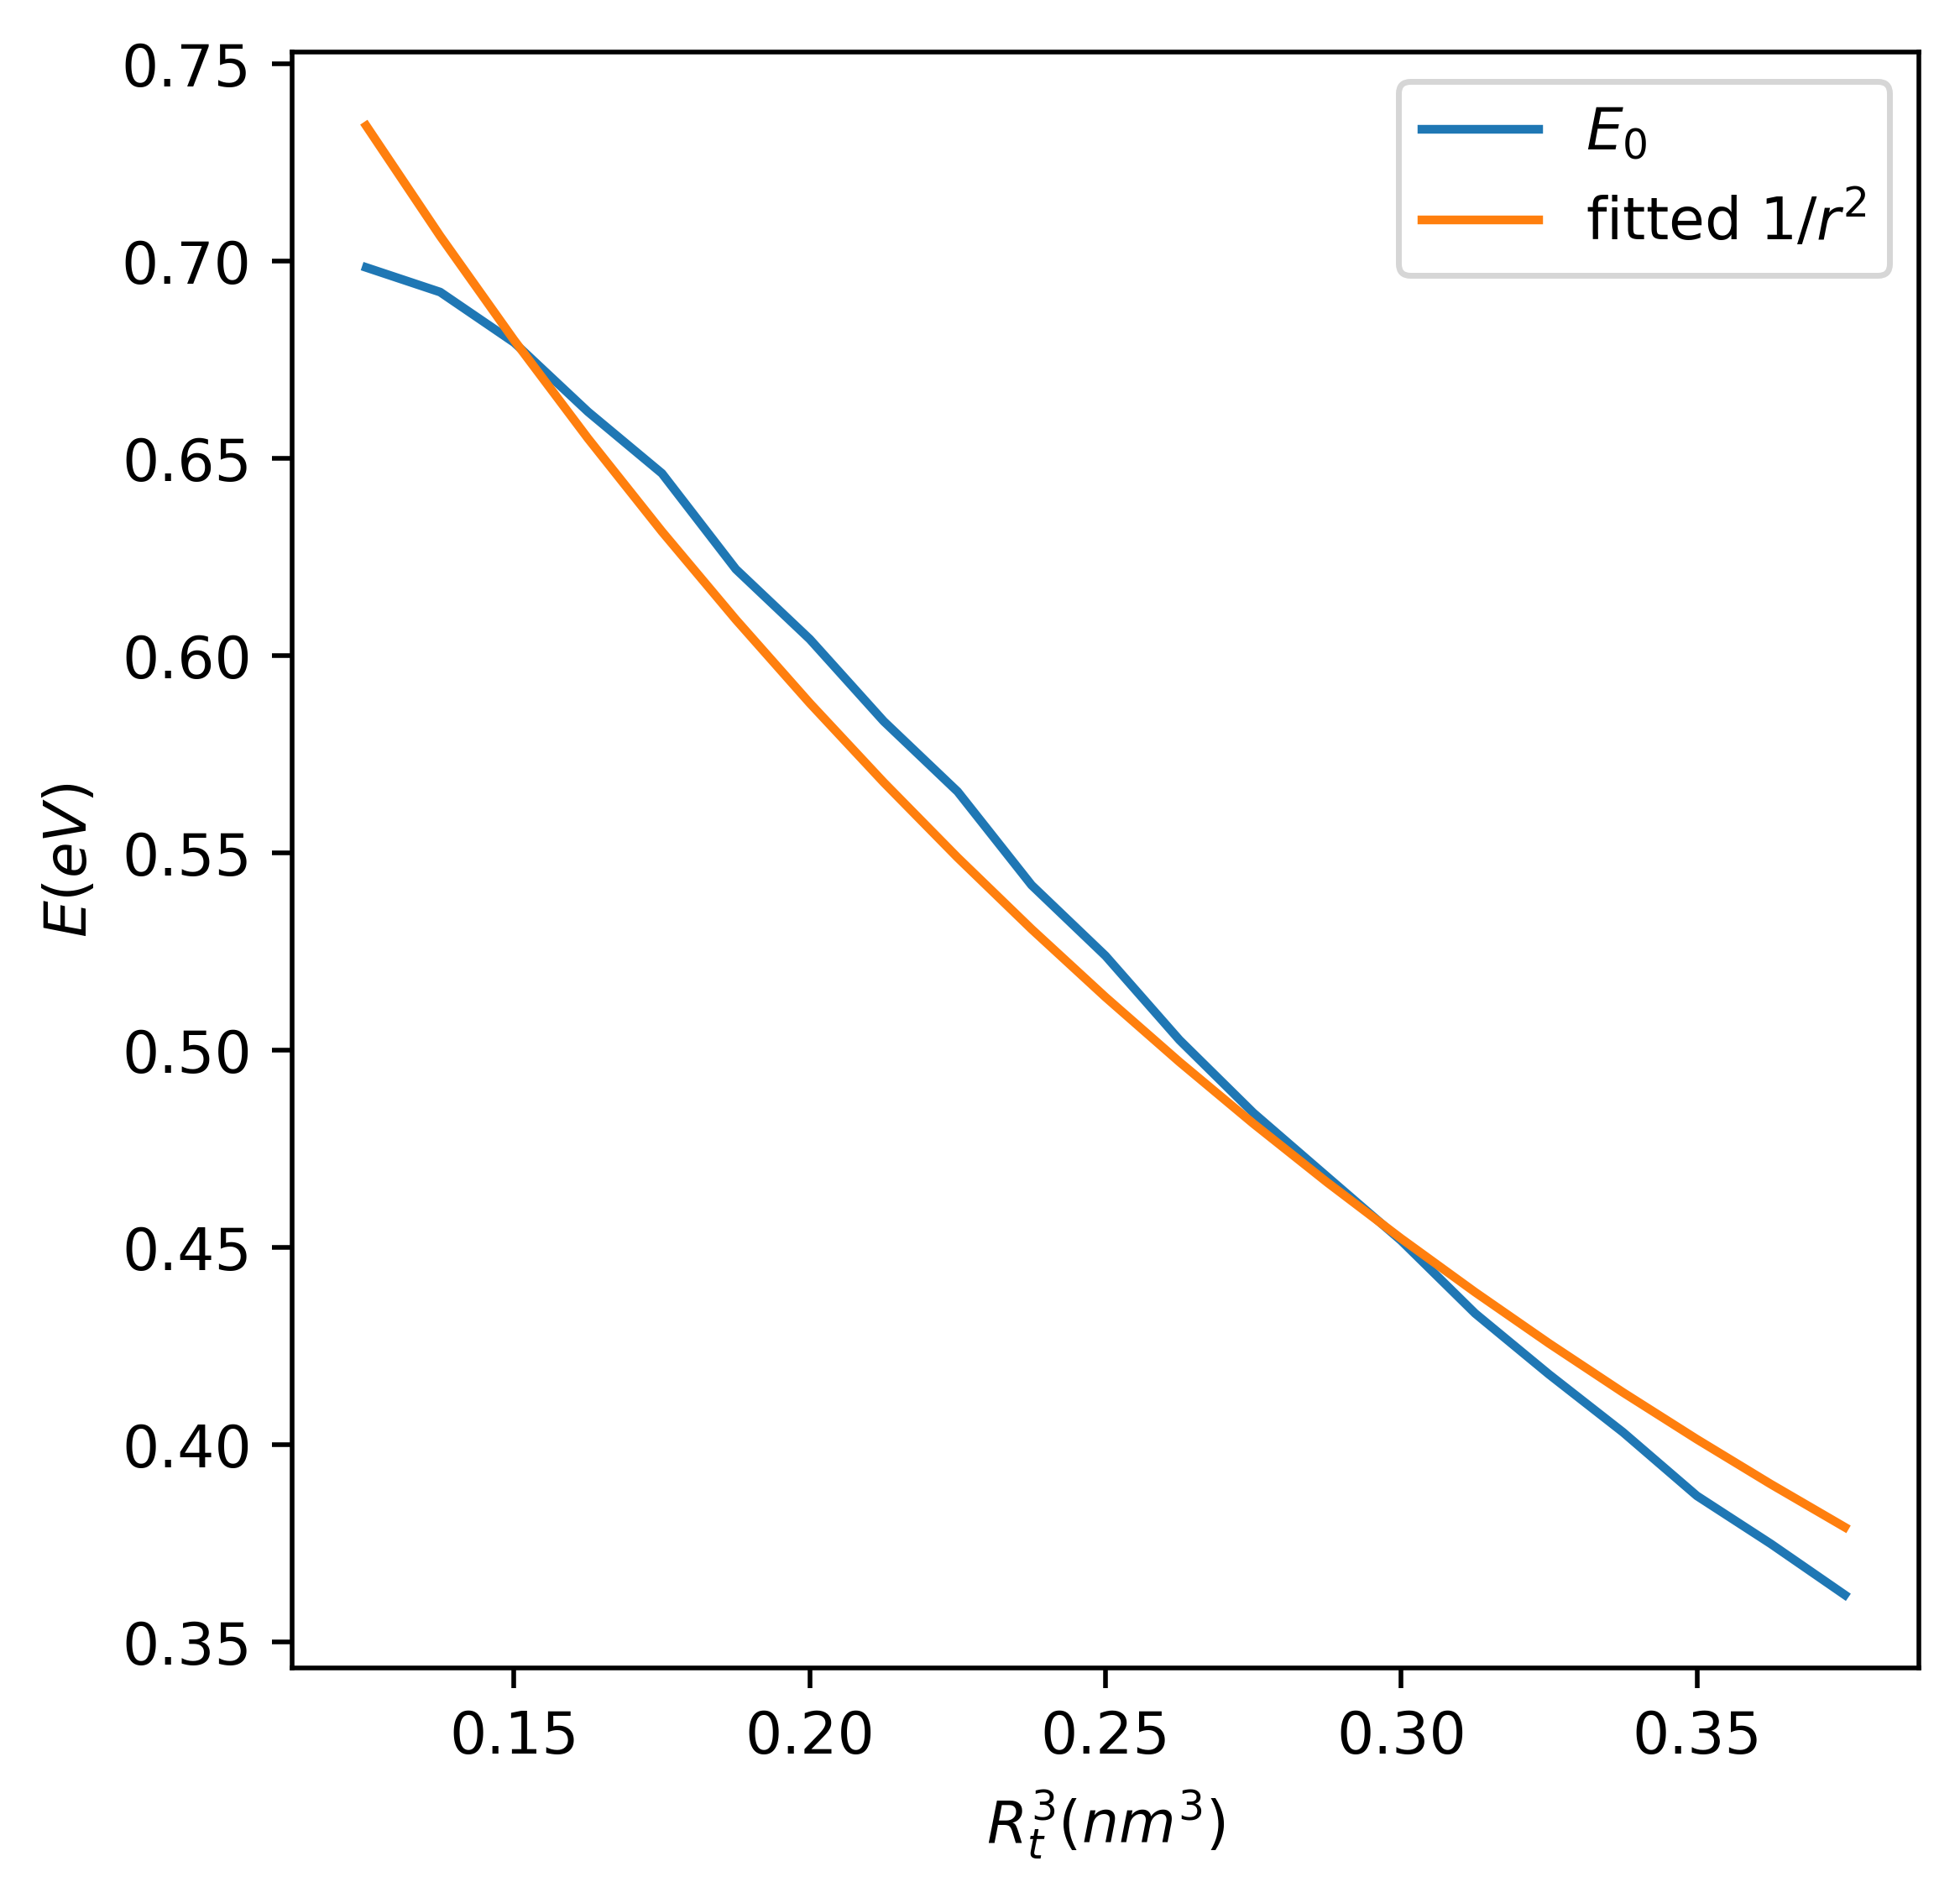
\includegraphics[scale = 0.5]{fit.png}
            \caption{fitting ground state energies}
            \label{fig: fitting}
        \end{figure}

    
    \subsection{Energy dependence in $m_{eff}$}

    one correction that could be made is to introduce energy dependence in the effective mass term:
    \begin{equation}
        H = -\frac{\hbar^2}{2}\nabla_r\left(\frac{1}{m(E, r)}\right)\nabla_r + V(r)
        \label{energy dependant mass schrodinger equation}
    \end{equation}

    where $m(E, r)$ is given by:
    \begin{equation}
        \frac{1}{m(E, r)} = \frac{P^2}{\hbar^2} \left( \frac{2}{E + E_g(r) - V(r)} + \frac{1}{E + E_g(r) + \Delta(r) - V(r)} \right)
        \label{effictive mass}
    \end{equation}
    Where $E_g(r)$ and $\Delta r$ denote, respectively, the band gap and the spin-orbit splitting in the valence band, and P is the momentum matrix element.\\
    This will introduce non-linearity to the Schrodinger equation, and it can be solved using an iterative non-linear scheme, which begins by selecting an initial energy value $E$. then the effective mass \( m(E, r) \) is computed using the energy $E$ as a parameter. Next, the Schrodinger equation is solved using the energy $E$ to obtain the corresponding wave functions and eigen-energies. After solving the Schrodinger equation, the energy value is updated to the corresponding eigen-energy and the process is repeated and the effective mass is recalculated with the updated energy value. This iterative process continues until convergence.
    
    % \color{red}
    % Here I should attempt the algorithm in my python code.
    % \color{black}
    
    \subsection{DFT}
    In the aforementioned methods we discussed the shape of the dot was assumed to be uniform, and the surface impurities (or missing atoms) were neglected. However, as the dot size get smaller and smaller these methods (even more suffocated ones such as $\mathbf{k\cdot p}$ perturbation theory) will fail to take into account the impurities in the surface, furthermore,  It is clear that the Quantum dot system includes electron-electron interaction between valence electrons, which makes it a many body problem, therefore it is convenient to use Many particle system Hamiltonian, and related models and theories to model QDs. The experimentally proven stability, as well as the small size of these systems allows for calculations of both ground and
    excited state properties by First-principles quantum methods such density functional theory (DFT) and time dependant density functional theory (TDDFT) with reasonable degree of accuracy. using optical and mass microscopy to determine the QD surface geometry, then using DFT to calculate related properties.\\
    Using these First principle models it was shown in \cite{kilina2016surface} that metals enriched QDs enhance the emission of the QDs by delocalized surface-associated orbitals than in Nonmetallic-enriched ($Cd_{34}S_{32}$ vs. $Cd_{32}S_{34}$) QDs, see figure \ref{fig:DFT metallic vs nonmetalic}.
    The effect of capping was also shown to be not always enhancing (when defects are introduced), since hole-leakage could occur, creating states close to the (VB) edge and affecting the optical properties. It was also shown that neutral ligands (amines,phosphines, and phosphine oxides) do not contribute to states near the energy gap of CdSe msQDs making them optically inactive.
    \begin{figure}
        \centering
        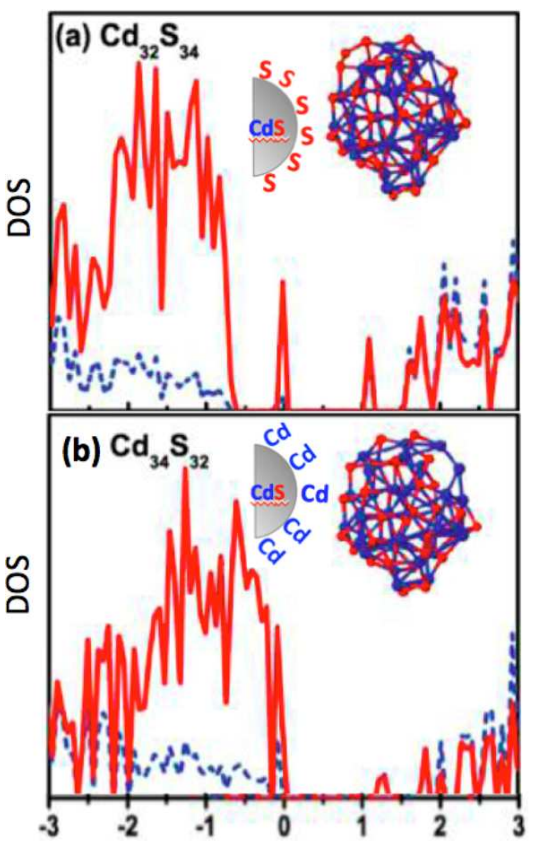
\includegraphics[scale = 0.4]{Dos metallic vs nonmetalic.png}
        \caption{$Cd_{34}S_{32}$ vs. $Cd_{32}S_{34}$ density of states}
        \label{fig:DFT metallic vs nonmetalic}
    \end{figure}

    DFT is also useful for studying the Coulomb blockade related effects, such as the peak spacing in the conductance through the dot, by comparing ground state energies as a function of the number of electrons in the dot\cite{sDFT}, as well as simulating the one electron transistor
    % One effecient and accurate model is the Kohn-Sham spin-Density Functuional Theorem (KS-SDFT), even though density functional theory gives approximations only to the ground states density and energies, it can be used to study other interesting properties of quantum dots, such as the conductance peak spacing through quantum dots.\\
    \subsection{Other Methods}
    Other methods such as $\mathbf{k\cdot p}$ perturbation theorey, Hatree Fock theory, and Monte-Carlo calculations.

\section{Experimental Results}
    \subsection{Testing methods}
    There are many interesting properties to study in the Quantum dots, such as energy, size and geometry, and legends or defections in the shape or type. To which many experimental methods might be used (such as STM for the shape and size of the dots). However, In this paper is more focused on energy manipulation, and therefore I will focus on the experimental calculations for energy gap calculations. Other than the UV/vis-spectroscopy. Photoluminescence (and its variations) and Cyclic Voltammetery have been used to study the energy structure of QDs.
        
        \subsubsection{photoluminescence (PL \& PLE)}
        In general, these two methods are often used to study energy spectra's of the materials, \textbf{PLE} is also known for its use on quantum wells. However, In the case of \textbf{QDs} it is sensitive to phonon emissions (That is, the case were the excited electrod does not relax to ground state directly). Furthermore, It has been shown that the the carrier relaxation efficiency is a function of energy, and therefore, \textbf{PLE} will resonate at multiples of phonon energy, for energies higher than the first transition energy, notable peaks appear at multiples of phonon energies, and when the difference between the incident and detected energy for different detected energies, further supporting the claim that these peaks correspond to phonons and proving the "non-ideal" relaxation of quatum dots, unlike atoms. Nevertheless, PL and PLE are still useful in studying dots relaxation mechanisms and their photon and phonon emissions can be indicators of the size distribution. \cite{steer1996electronic}

        \subsubsection{CV}
        CV test can also be used to analyze the energy gap of the Quantum dot, or  valence band edge and conduction band edge (due to confinement), the hole energy at top of valance band and the electron energy at the edge of conduction band are shown to be proportional to respective cathodic and anodic peaks in the CVs. Hence, the difference in voltage will be directly correlated to the dot's band gap, therefore it is expected that as the Q-dot size decreases, the cathodic and anodic peaks shift to higher energies, and away from each other (so to increase the gap energy). Figure \ref{fig:CV} shows this for different QDs sizes. Where, for example, the energy gap in the dot (F) was found to be $2.40$e$V$ which agrees with the difference between the $2$ blue lines in the figure, in fact, for all samples the CV calculations highly agrees with the UV/Vis spectroscopy for the shown samples, with differences not exceeding $0.01$ e$V$.\cite{haram2011quantum}


        \begin{figure}[h]
            \centering
            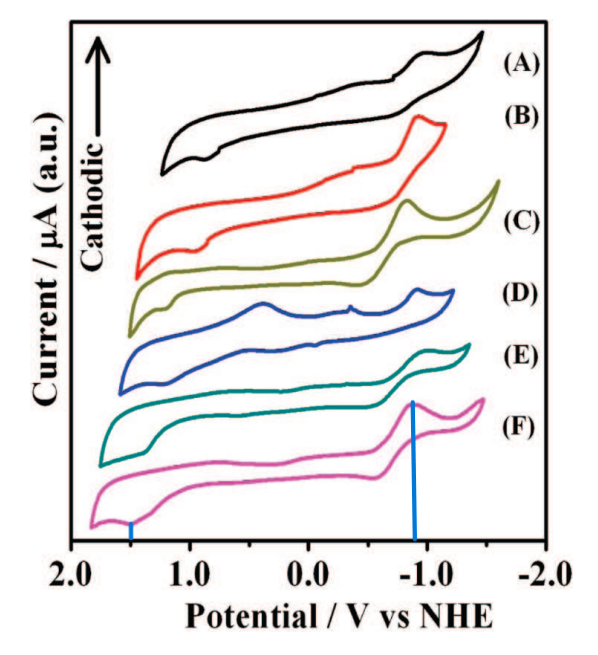
\includegraphics[scale=0.4]{CV_QDs.png}
            \caption{CVs for varias QDs samples, with varying sizes. The figure is from \cite{haram2011quantum}}
            \label{fig:CV}
        \end{figure}
            
        

    \subsection{Energy Tuning}
    There are many properties that contribute to the energy levels of quantum dots, those properties include size, shape and geometry, material type and strain. However, from an experimental and manufacturing point of view, there properties are controlled by certain parameters, such as the amount of strain material deposited, an anneal time and deposition rate and growth temperature.

        \subsubsection{Growth temperature}
         The shell structure can be tuned by adjusting the substrate temperature during the formation of the QD’s. Larger QD’s with smaller band gap energies are obtained at higher growth temperatures, however, the size is not the only factor that is affected by the growth temperature, the intermixing between QDs is also reduced when the growth temperature is lowered, thus increasing the uniformity of the QD. \cite{fafard1999manipulating}

        \subsubsection{QD density}
        To obtain uniform QD’s with well-defined energy levels, the QD density has to be kept low, indium coverage should also be optimized, for low coverage below $1.8$ \textbf{ML} only wetting layer will be observed in the energy spectroscopy (InAs islands are not formed) while in the case of indium coverage higher than $1.9$ \textbf{ML} the energy levels will intersect, and confinement effect will tend to vanish due to the higher probability of island coalescence. The optimal value for indium coverage was shown to be $1.84$ \textbf{ML}.\cite{fafard1999manipulating}
        
        \subsubsection{Thermal Annealing}
         tuning of the QD interband transition energy can be achieved using by rapid thermal annealing (RTA), depending on annealing time and temperature. RTA has the effect of blue-shift, narrowing (PL) line-width and decrease in the intersublevel spacing energies as the annealing temperature increases. Annealing time is also an important factor.\\TEM images shows that the QD's size does not change significantly with RTA, the change in the energy levels is attributed to the increase of Ga concentration in QDs due to the inter-diffusion of In–Ga atoms at the interface between the QD and the GaAs barrier. The increase of Ga concentration will increase the energy gap and decrease the potential difference (barrier potential) between the QD and the GaAs barrier.\cite{hsu2000tuning}

\section{Future: Graphene Quantum Dots}
    The 2D structure of the graphene opens the gates to different solid state applications, Quantum dots are no exception. The Graphene Quantum dots (GQD) have been hypothesized and studied more and more in the recent years.
    \subsection{Theory}
    Theoretical treatment to the assumed Graphene quantum dots shows some interesting results:
    \begin{enumerate}
        \item In contrast to conventional semiconductor quantum dots where the ground state is localized at the center of dot, the ground states for the conduction and valence bands localize at the middle of each edge in the Hexagonal Graphene structure. \cite{zhang2008tuning}
        
        \item As expected, the energy gap decreases as the size of the GQD increases, however, with some types of GQDs, the proportionality is $\Delta E \prop 1/L$ which is different from the conventional case, and marks the possibility to produce bigger quantum dots where confinement is still possible.\cite{zhang2008tuning}
    \end{enumerate}

    \subsection{Experiments}
    In the experimental realm, the existence and whether GCDs have been made is still a matter of dispute, some papers claim that they have successfully made GCDs at laboratories\cite{silvestrov2007quantum}, others argue that are these are rather fluorescent organic dots not 2D Graphene ones.\cite{pu2018colloidal}

\section*{Appendicies}
    \subsection*{A: Kohn-Sham Density Functional Theorem (KS-DFT)}
        Here, I will present a brief overview of (DFT) as was explained by \cite{sDFT}.\\
        The Kohn-Sham Hamiltonian is given by:
        \begin{equation}
            \hat{H}^\sigma = -\frac{1}{2} \nabla^2 + V^\sigma_{\text{ext}}(\mathbf{r}) + V^\sigma_{\text{H}}(\mathbf{r}) + V^\sigma_{\text{XC}}(\mathbf{r})
            \label{KSSDFT hamiltonian}
        \end{equation}
        
        where $\sigma \in \{\alpha\text{, }\beta\}$ is the spin, and $V_{\text{XC}}$ is the exchange-correlation potential, which is purely a quantum term in the Hatree operator resulting from the anti-symmetric behaviour of fermions. While the Hatree potential is given by $E\int \frac{n(\mathbf{r})}{\left|\mathbf{r} - \mathbf{r'}\right|} \, d\mathbf{r}$.
        
        The energy functional is therefore given by:
        \begin{equation}
            E[n^\alpha(\mathbf{r}), n^\beta(\mathbf{r})] = T[n^\alpha(\mathbf{r}), n^\beta(\mathbf{r})] + \int_{\mathbf{r}} n(\mathbf{r}) V_{\text{ext}}(\mathbf{r}) \, d\mathbf{r} + \int_{\mathbf{r}}\int_{\mathbf{r'}} \frac{n(\mathbf{r})n(\mathbf{r'})}{\left|\mathbf{r} - \mathbf{r'}\right|}\, d\mathbf{r} d\mathbf{r'} + E_{\text{XC}}[n^\alpha(\mathbf{r}), n^\beta(\mathbf{r})]
        \end{equation}
        
        where $n^\sigma(\mathbf{r})$ is the density of spin orbitals, and it is given by:
        \begin{equation}
            n^\sigma(\mathbf{r}) = \sum_i^{N^\alpha} \left|\psi^\sigma_i(\mathbf{r})\right|^2
            \label{density}
        \end{equation}
        
        $T[n^\alpha(\mathbf{r}), n^\beta(\mathbf{r})]$ represents the kinetic energy, and is given as $-\frac{1}{2}\sum_{i, \sigma} \langle \psi_i ^\sigma \vert \nabla^2 \vert \psi_i^\sigma\rangle$. Where $\left\{\psi_i^ \sigma( \mathbf{r}) \right\}$ are the single electron states (the eigen functions are represented as by their Hatree product). And they are obtained from:
        \begin{equation}
            \hat{H}^\sigma\vert\psi_i^\sigma(\mathbf{r})\rangle = \epsilon_i^\sigma \vert\psi_i^\sigma(\mathbf{r})\rangle
        \end{equation}
        
        Therefore, in order to solve for the single orbital states, the Hatree potential requires the knowledge of the density, and similarly, the density depends on the single orbital states, therefore an iterative scheme will be used, in which a set of trial functions $\left\{\psi_i ^\sigma (\mathbf{r}) \right\}$ will be assumed and then updated based on the Energy values, until energy convergence is achieved.\\
        A problem with the (DFT) is the lack of an exact way to calculate $E_{\text{XC}}$, for this sake, multiple methods have been used to approximate it, such as the spin-polarized uniform electron gas exchange energy functional, local-spin-density approximation (LSDA).\\

        

\newpage
\vskip 0.2in
\bibliographystyle{abbrv}
\bibliography{references}

\end{document}
